\documentclass[11pt,a4paper]{article}
\usepackage[utf8]{inputenc}
\usepackage[T1]{fontenc}
\usepackage[brazil]{babel}
\usepackage{geometry}
\usepackage{graphicx}
\usepackage{booktabs}
\usepackage{longtable}
\usepackage{array}
\usepackage{float}
\usepackage{xcolor}
\usepackage{listings}
\usepackage{pdflscape}
\usepackage{placeins}
\usepackage[hidelinks]{hyperref}
\geometry{margin=2.1cm}
\setlength{\parskip}{0.5em}
\setlength{\parindent}{0pt}
\lstset{
  basicstyle=\ttfamily\footnotesize,
  breaklines=true,
  columns=fullflexible,
  frame=single,
  showstringspaces=false,
  keywordstyle=\color{blue},
  commentstyle=\color{gray}
}
\title{Relatório científico da matriz de capacidade do Apache Druid}
\author{CCO DataOps}
\date{30 de junho de 2026}
\begin{document}
\maketitle


\section{Como ler este documento}

Este relatório foi reorganizado para acompanhar o raciocínio experimental. Primeiro são descritos arquitetura e metodologia. Em seguida, cada métrica e cada gráfico são lidos explicitamente: o que medem, por que importam, como interpretar e o que os dados mostram nesta matriz. As tabelas extensas foram movidas para o apêndice operacional para não interromper a análise.

\section{Arquitetura experimental}

A avaliação considera apenas a camada OLAP de consulta do Apache Druid. O teste não executa Kafka, Superset, ingestão nem tabela fato. A pergunta experimental é: com as dimensões já carregadas, qual perfil de Broker/Historical sustenta consultas analíticas sem erro?

O hardware local observado possui 8 CPUs lógicas e aproximadamente 7.48 GiB de RAM. A disponibilidade instantânea durante a geração do relatório foi de 1.28 GiB. Esse contexto importa porque Druid usa memoria direta, heap e threads de processamento; em ambiente local, aumentar o perfil dos containers compete com o restante do sistema.

\begin{itemize}

\item \textbf{Broker}: planeja SQL, coordena fan-out e junta resultados. Ele sofre quando a consulta exige merge grande ou muitos joins.

\item \textbf{Historical}: varre segmentos persistidos e executa parte pesada das agregações. Foi o ponto de saturação nos cenários menores.

\item \textbf{Coordinator}: garante disponibilidade dos segmentos. Na matriz, seu papel foi validar loadstatus, não executar consulta.

\item \textbf{MiddleManager}: quase irrelevante neste experimento porque não houve ingestão.

\item \textbf{Router, Postgres, Zookeeper e Kafka}: dão suporte operacional, mas não aparecem como gargalo nos dados coletados.

\end{itemize}

\subsection{Perfis comparados}

{
\small
\setlength{\tabcolsep}{4pt}
\renewcommand{\arraystretch}{1.15}
\begin{longtable}{p{0.12\textwidth}p{0.08\textwidth}p{0.08\textwidth}p{0.10\textwidth}p{0.10\textwidth}p{0.42\textwidth}}
\caption{Perfis de capacidade aplicados ao Broker e ao Historical.}\\
\toprule
Cenario & CPU & GB & Threads & Merge & Trade-off \\
\midrule
\endfirsthead
\toprule
Cenario & CPU & GB & Threads & Merge & Trade-off \\
\midrule
\endhead
Baseline & 1.000 & 1.000 & 1 & 1 & Menor consumo; maior risco de saturação em joins concorrentes. \\
Balanced & 1.500 & 1.500 & 2 & 2 & Uso diário; melhora QPS em concorrência 2, mas ainda falha em concorrência 4. \\
Query Heavy & 2.000 & 2.000 & 3 & 3 & Maior consumo; único perfil estável na concorrência 4. \\
\bottomrule
\end{longtable}
}


Os três cenários alteram apenas os recursos dos nós de consulta, Broker e Historical. Isso preserva comparabilidade: os dados, queries, concorrências e modos cold/warm são os mesmos.

\clearpage

\section{Metodologia e métricas de leitura}

A matriz usa 19 queries, concorrências 1, 2 e 4, e duas condições de cache: cold-start e warm-start. Cada resultado deve ser lido combinando vazão, latência de cauda e erro. O erro tem prioridade interpretativa: um cenário com QPS alto e erro alto não é estável.

{
\small
\setlength{\tabcolsep}{4pt}
\renewcommand{\arraystretch}{1.15}
\begin{longtable}{p{0.28\textwidth}p{0.09\textwidth}p{0.11\textwidth}p{0.13\textwidth}p{0.10\textwidth}p{0.16\textwidth}}
\caption{Resumo compacto para leitura no relatorio principal.}\\
\toprule
Cenario & Conc. & QPS & p95 ms & Erros & Classe \\
\midrule
\endfirsthead
\toprule
Cenario & Conc. & QPS & p95 ms & Erros & Classe \\
\midrule
\endhead
Cenario 1 - Baseline & 1 & 1.489 & 2410.465 & 0 & ESTAVEL \\
Cenario 1 - Baseline & 2 & 2.882 & 3912.175 & 0 & ESTAVEL \\
Cenario 1 - Baseline & 4 & 0.952 & 2054.123 & 14 & SATURADO \\
Cenario 2 - Balanced & 1 & 2.144 & 2733.528 & 0 & ESTAVEL \\
Cenario 2 - Balanced & 2 & 4.408 & 2547.336 & 0 & ESTAVEL \\
Cenario 2 - Balanced & 4 & 1.350 & 1038.265 & 17 & SATURADO \\
Cenario 3 - Query Heavy & 1 & 2.673 & 2049.782 & 0 & ESTAVEL \\
Cenario 3 - Query Heavy & 2 & 5.136 & 2403.284 & 0 & ESTAVEL \\
Cenario 3 - Query Heavy & 4 & 3.770 & 6422.163 & 0 & ESTAVEL \\
\bottomrule
\end{longtable}
}


A tabela compacta acima é a âncora numérica do relatório. Ela mostra que o Baseline e o Balanced passam a falhar em concorrência 4, enquanto o Query Heavy mantém erro zero, ainda que com p95 maior.

\subsection{Resumo das métricas usadas}

\begin{itemize}

\item \textbf{QPS}: vazão de consultas finalizadas por segundo.

\item \textbf{p95/p99}: latência de cauda; mostram como o sistema se comporta para usuários menos favorecidos pela distribuição.

\item \textbf{Taxa de erro}: falhas HTTP, timeouts ou desconexões. Erro invalida comparação puramente por latência.

\item \textbf{Cold/warm}: aproxima diferença entre consulta fria e consulta repetida com cache.

\item \textbf{CPU/memória Docker}: evidência operacional do gargalo em Broker/Historical.

\end{itemize}

Definições completas estão no PDF \texttt{guia\_metricas\_benchmark.pdf}.

\section{Throughput: QPS por cenário}

\textbf{O que mede.} QPS mede quantas consultas completas o sistema entrega por segundo dentro de cada nível de concorrência.

\textbf{Por que importa.} Em painéis Superset, vários cards podem disparar consultas simultâneas. Um perfil útil precisa aumentar vazão sem perder confiabilidade.

\textbf{Como interpretar.} A curva ideal cresce com concorrência até o ponto de saturação. Queda de QPS com aumento de concorrência indica contenção, erro ou reset de conexão.

\begin{figure}[H]\centering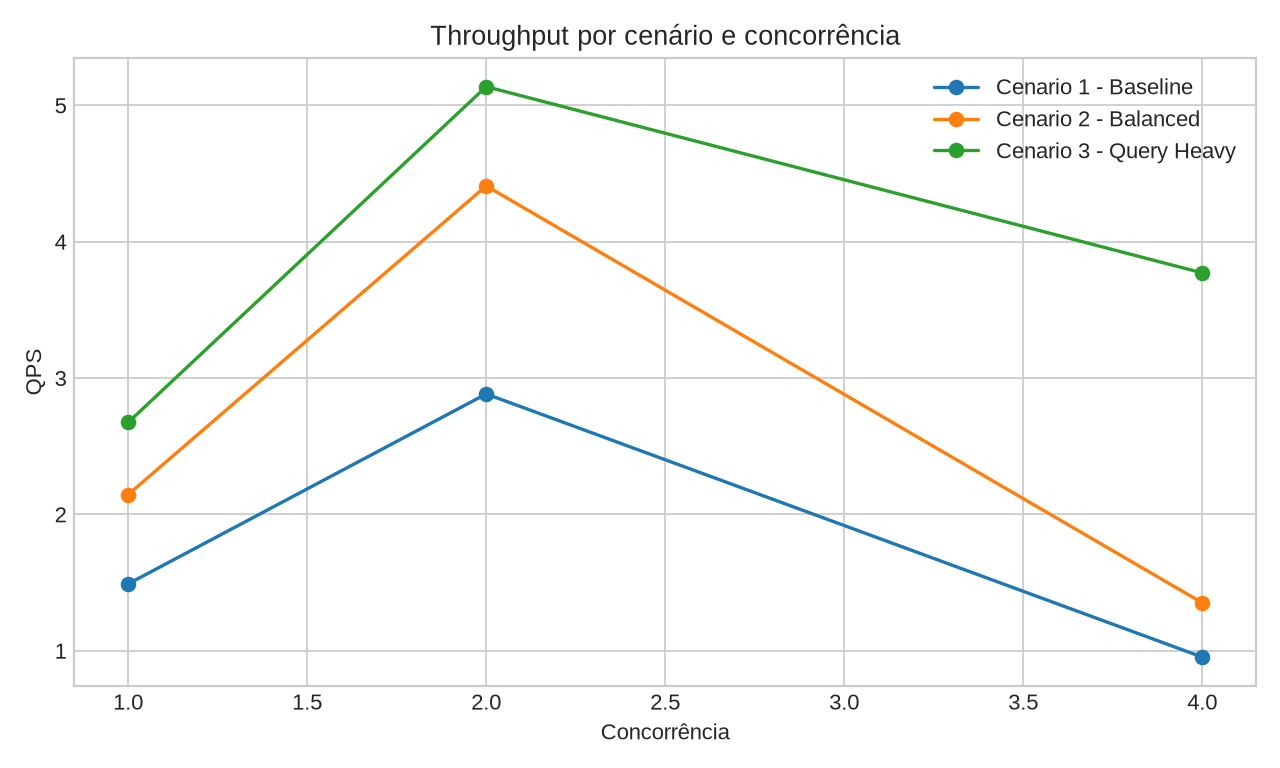
\includegraphics[width=0.92\textwidth,height=0.42\textheight,keepaspectratio]{../figures/qps_por_concorrencia.png}\caption{Throughput por cenário e concorrência.}\label{fig:qps}\end{figure}

\textbf{Leitura dos dados.} O Balanced atinge 4.408 QPS em concorrência 2, melhor que o Baseline no mesmo ponto. Em concorrência 4, porém, o Query Heavy chega a 3.770 QPS com erro zero, enquanto Baseline e Balanced caem para 0.952 e 1.350 QPS com falhas.

\FloatBarrier

\section{Latência de cauda: p95 e p99}

\textbf{O que mede.} p95 e p99 mostram a cauda de resposta. Eles respondem: quão ruim fica para as consultas mais lentas que ainda completam?

\textbf{Por que importa.} Dashboards operacionais sofrem mais com cauda longa do que com média. Uma tela pode ficar bloqueada esperando a consulta mais lenta.

\textbf{Como interpretar.} Latência alta sem erro indica custo real de processamento. Latência baixa com erro alto pode ser enganosa, pois parte das consultas nem terminou.

\begin{figure}[H]\centering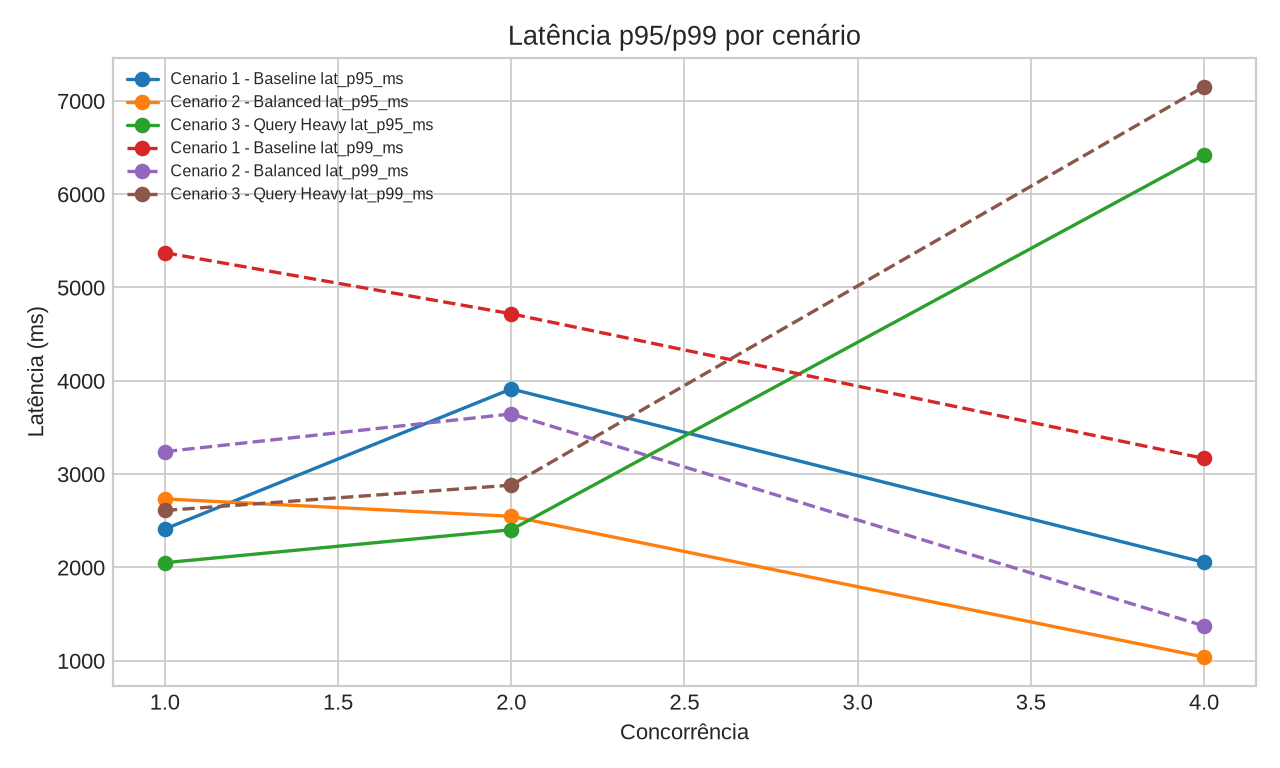
\includegraphics[width=0.92\textwidth,height=0.42\textheight,keepaspectratio]{../figures/latencia_p95_p99.png}\caption{Latência p95/p99 por cenário.}\label{fig:latencia}\end{figure}

\textbf{Leitura dos dados.} O Query Heavy em concorrência 4 tem p95 de 6422.163 ms e p99 de 7152.003 ms. Esse valor é alto, mas representa consultas concluídas. No Baseline e Balanced, a leitura de p95 em concorrência 4 deve ser subordinada à taxa de erro, pois houve perda de requisições.

\FloatBarrier

\section{Erro e saturação}

\textbf{O que mede.} A taxa de erro mede falhas reais observadas pelo cliente SQL. A classe SATURADO marca cenários em que erro ou limites operacionais invalidam estabilidade.

\textbf{Por que importa.} Em banco OLAP, falha intermitente é pior do que latência previsível: o usuário não recebe resultado e o painel pode quebrar.

\textbf{Como interpretar.} Qualquer barra acima de zero em benchmark pequeno deve ser tratada como evidência de limite operacional.

\begin{figure}[H]\centering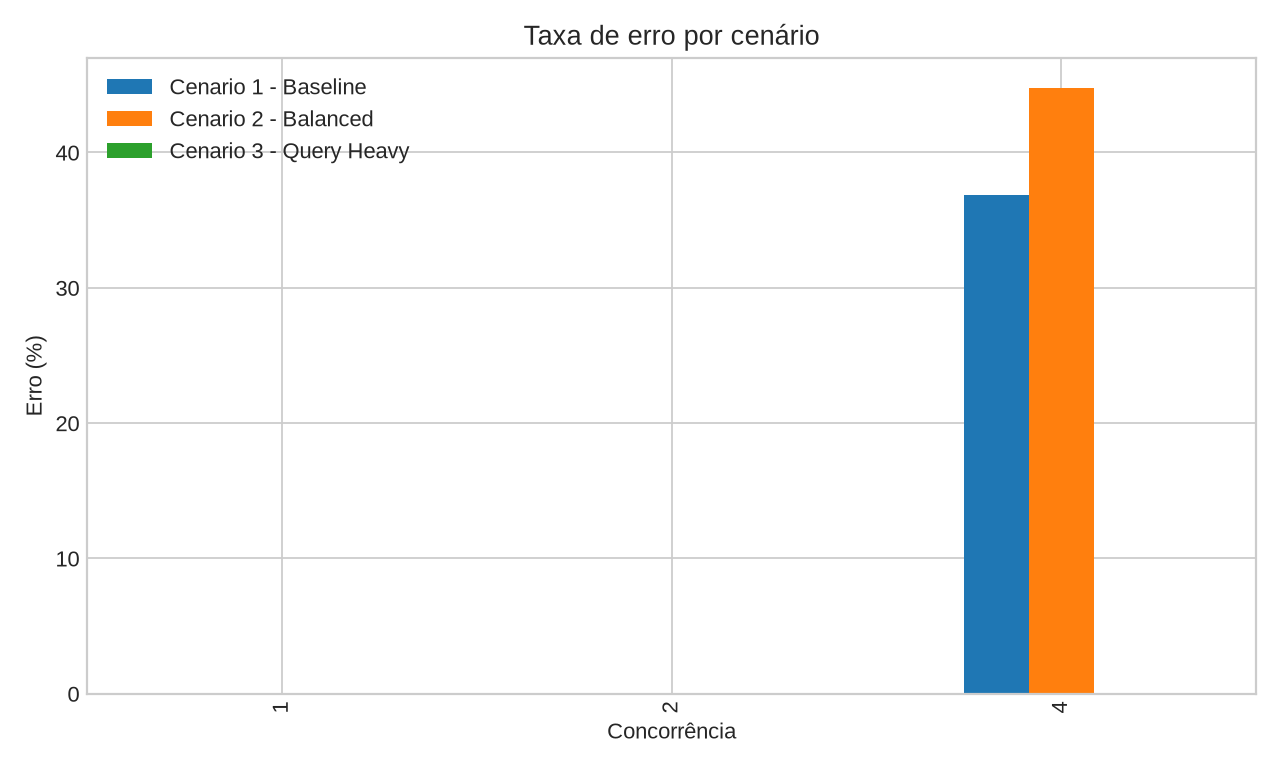
\includegraphics[width=0.92\textwidth,height=0.42\textheight,keepaspectratio]{../figures/taxa_erro.png}\caption{Taxa de erro por cenário.}\label{fig:erro}\end{figure}

\textbf{Leitura dos dados.} Baseline em concorrência 4 registrou 14 erros (36.842\%). Balanced registrou 17 erros (44.737\%). Query Heavy manteve 0 erro.

\FloatBarrier

\section{Evidência operacional: CPU e memória}

\textbf{O que mede.} O gráfico compara picos de CPU e memória nos containers Broker e Historical.

\textbf{Por que importa.} Se a falha vem do Historical, aumentar apenas Broker não resolveria. A evidência operacional indica onde a carga encosta.

\textbf{Como interpretar.} CPU acima de 100\% indica uso de mais de um core lógico. Memória percentual menor em cenários maiores pode refletir limite maior, não menor consumo absoluto.

\begin{figure}[H]\centering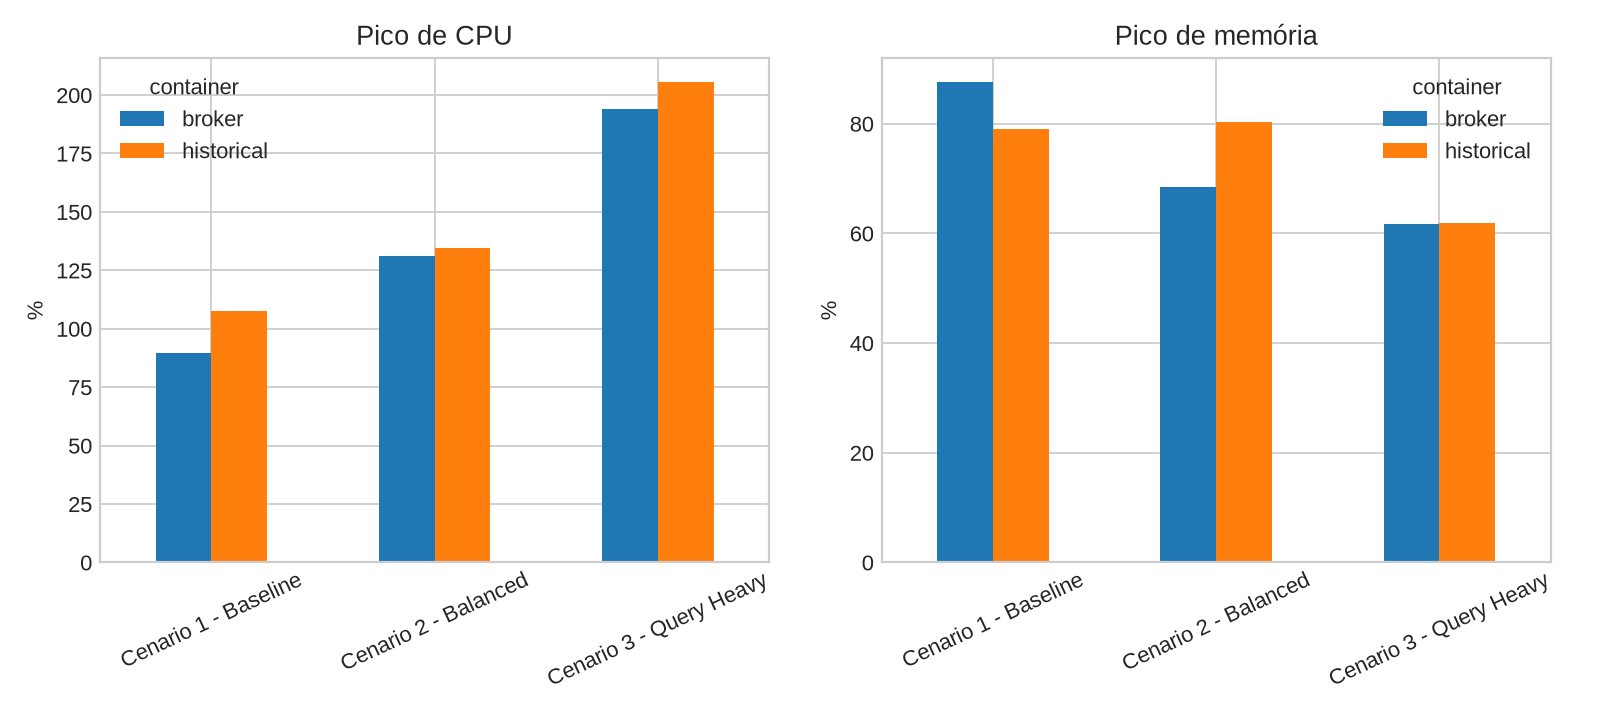
\includegraphics[width=0.92\textwidth,height=0.42\textheight,keepaspectratio]{../figures/docker_cpu_mem_picos.png}\caption{Picos de CPU e memória em Broker e Historical.}\label{fig:docker}\end{figure}

A leitura operacional sustenta a interpretação: Query Heavy usa mais CPU em Broker e Historical, mas transforma recurso adicional em estabilidade. Baseline e Balanced falham antes de sustentar concorrência 4.

\FloatBarrier

\section{Cold-start, warm-start e hotspots}

\textbf{O que mede.} O ganho warm-start compara consultas frias e consultas repetidas com cache. O heatmap mostra quais queries concentram p95 alto.

\textbf{Por que importa.} Superset costuma repetir consultas parecidas quando filtros e painéis são usados. Cache ajuda, mas não substitui capacidade quando há joins pesados.

\textbf{Como interpretar.} Ganho de cache deve ser lido por query. Joins dimensionais podem continuar caros mesmo com cache, porque o custo de planejamento, merge e cardinalidade permanece.

\begin{figure}[H]\centering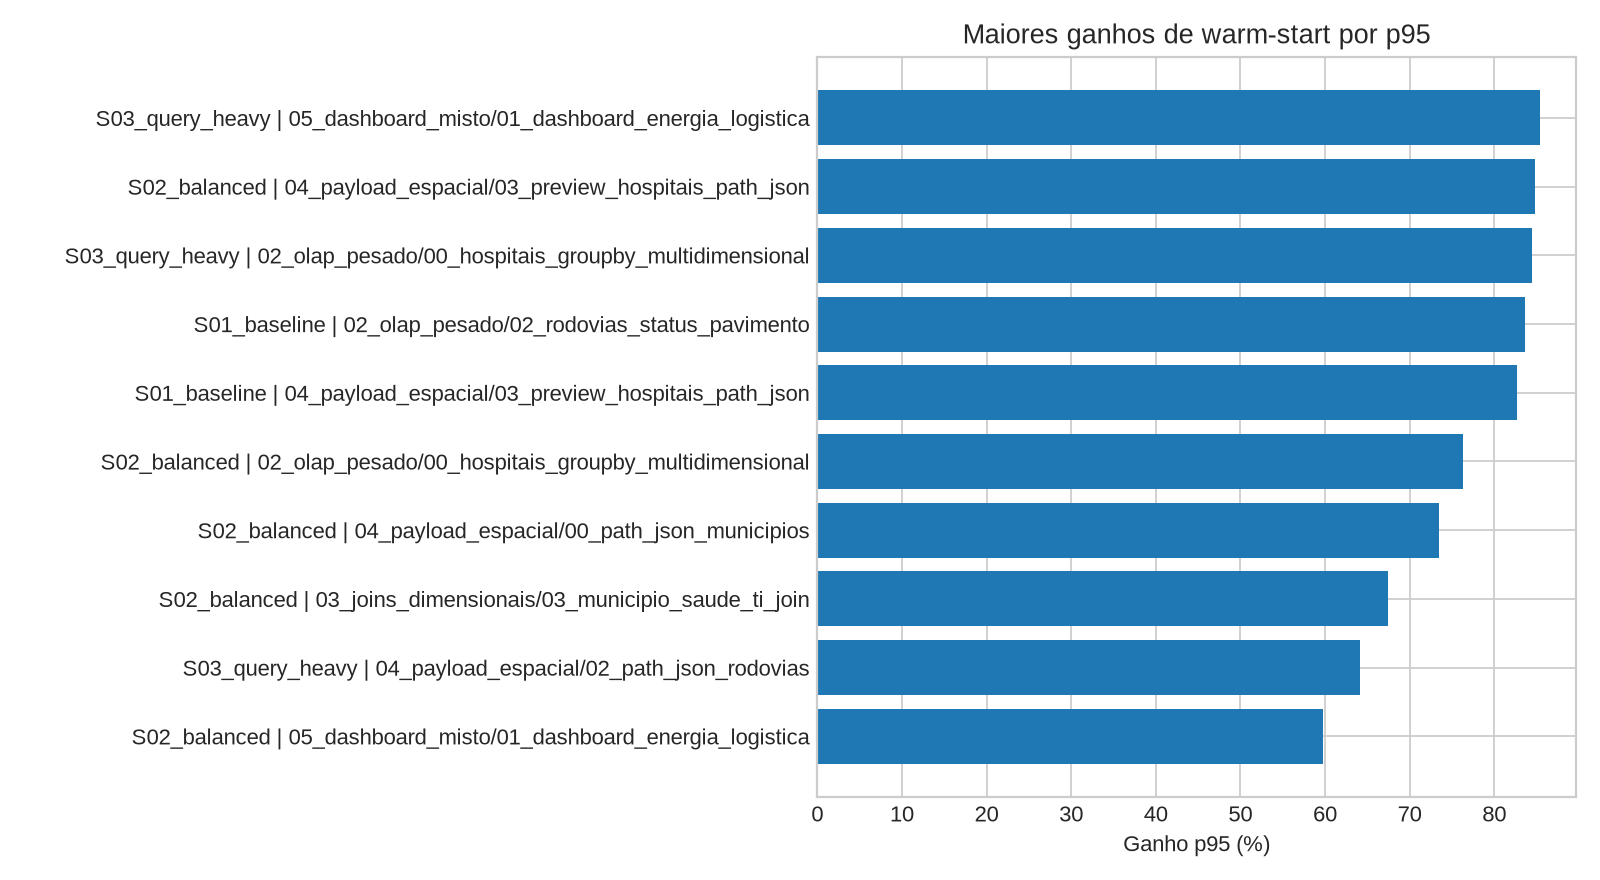
\includegraphics[width=0.92\textwidth,height=0.42\textheight,keepaspectratio]{../figures/ganho_warm_start_top10.png}\caption{Maiores ganhos de warm-start por p95.}\label{fig:warm}\end{figure}

\begin{figure}[H]\centering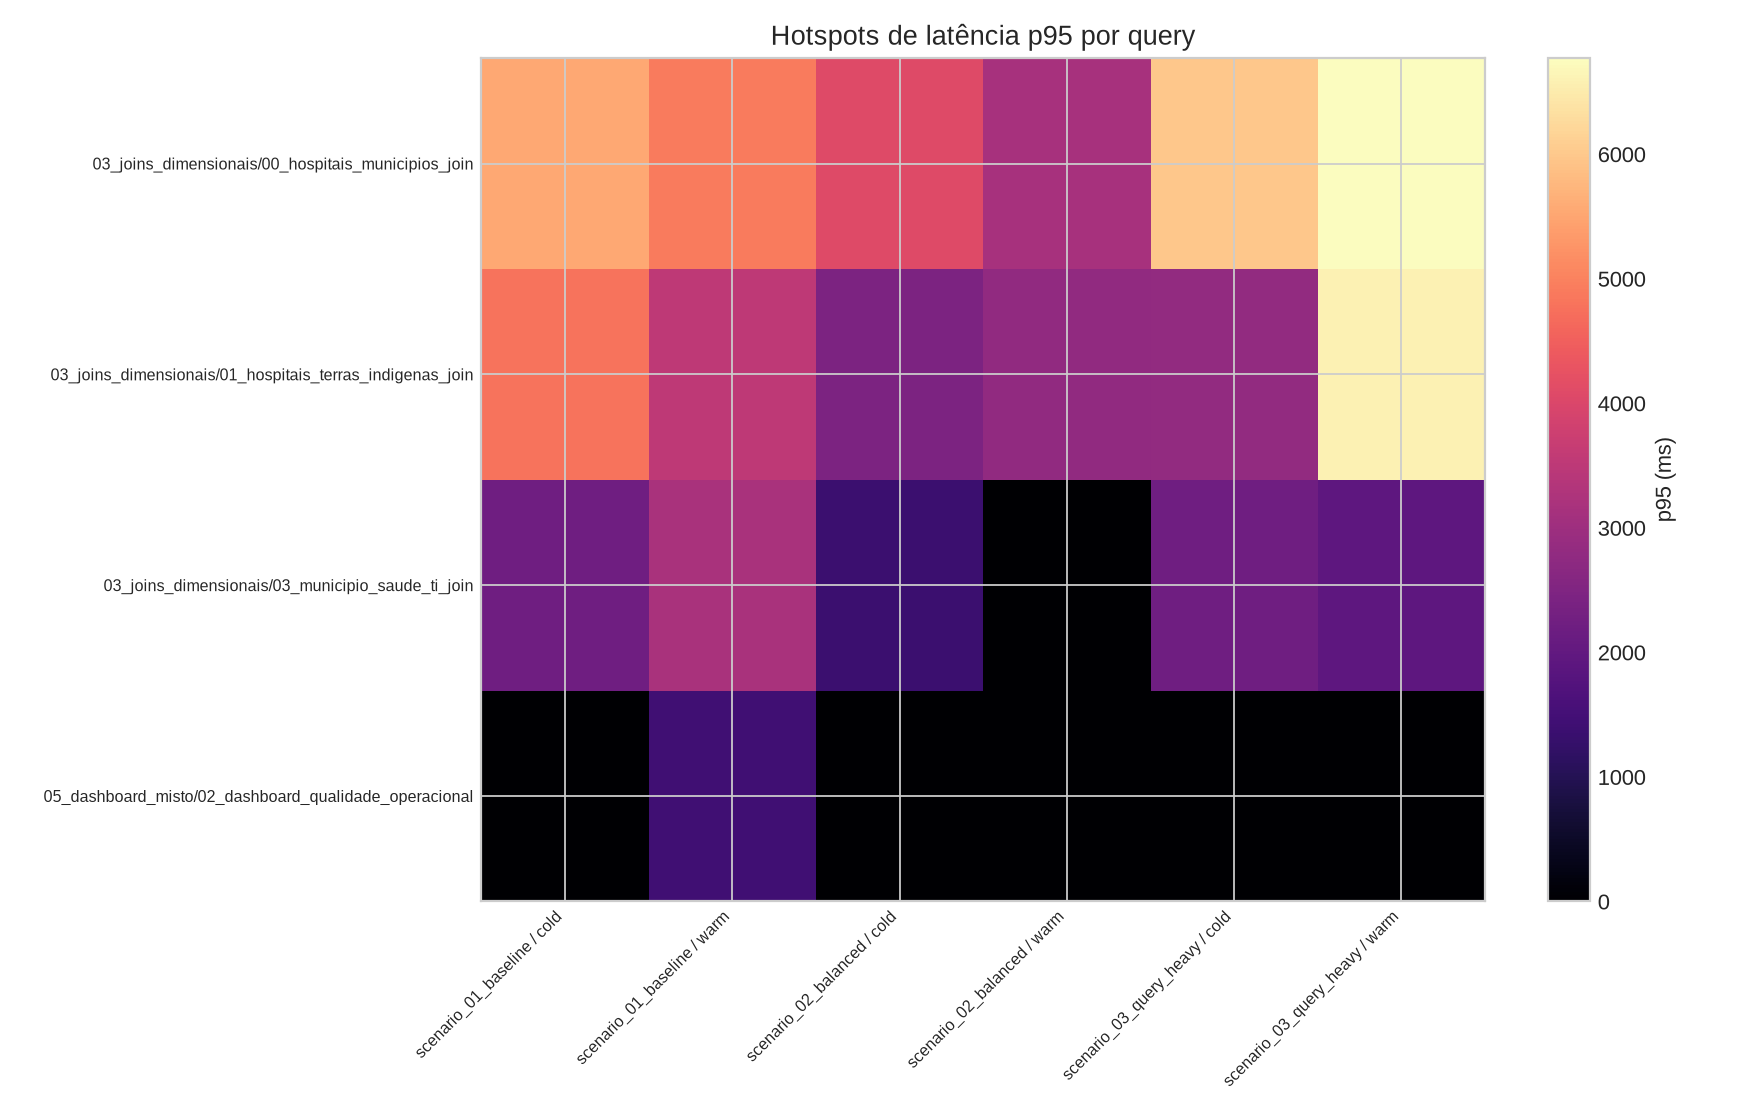
\includegraphics[width=0.92\textwidth,height=0.42\textheight,keepaspectratio]{../figures/heatmap_hotspots_queries.png}\caption{Hotspots de latência p95 por query, cenário e cache.}\label{fig:hotspots}\end{figure}

Os hotspots se concentram nos joins dimensionais com hospitais, municípios e terras indígenas. Isso confirma que o gargalo não é apenas o volume de `path_json`, mas o cruzamento analítico sobre a maior dimensão.

\FloatBarrier

\section{Interpretação técnica}

A comparação mostra que o perfil Query Heavy e o primeiro perfil estável para a carga avaliada. O Balanced é melhor para uso diário moderado, especialmente em concorrência 2, mas ainda não sustenta concorrência 4. O Baseline é útil como configuração econômica e controle experimental, não como perfil robusto para dashboards concorrentes.

A conclusão não é que Druid seja lento; é que o par Broker/Historical precisa ser dimensionado de acordo com o tipo de consulta. Para dimensões batch e queries OLAP com joins, o Historical precisa de CPU e memória direta suficientes para varrer segmentos e manter canais estáveis.

\section{Rastreabilidade}

A matriz analisada está em \texttt{data/results/performance/druid\_capacity/20260630\_000802}. Este relatório foi gerado a partir dos CSVs e JSONs ja consolidados, sem executar novo benchmark.


\end{document}
